\documentclass{beamer}

%
% Choose how your presentation looks.
%
% For more themes, color themes and font themes, see:
% http://deic.uab.es/~iblanes/beamer_gallery/index_by_theme.html
%
\mode<presentation>
{
  \usetheme{default}      % or try Darmstadt, Madrid, Warsaw, ...
  \usecolortheme{default} % or try albatross, beaver, crane, ...
  \usefonttheme{default}  % or try serif, structurebold, ...
  \setbeamertemplate{navigation symbols}{}
  \setbeamertemplate{caption}[numbered]
  \setbeamertemplate{footline}[page number]
  \setbeamercolor{frametitle}{fg=white}
  \setbeamercolor{footline}{fg=black}
} 

\usepackage[english]{babel}
\usepackage[utf8x]{inputenc}
\usepackage{tikz}
\usepackage{listings}
\usepackage{courier}

\xdefinecolor{darkblue}{rgb}{0.1,0.1,0.7}
\xdefinecolor{dianablue}{rgb}{0.18,0.24,0.31}
\definecolor{commentgreen}{rgb}{0,0.6,0}
\definecolor{stringmauve}{rgb}{0.58,0,0.82}

\lstset{ %
  backgroundcolor=\color{white},      % choose the background color
  basicstyle=\ttfamily\small,         % size of fonts used for the code
  breaklines=true,                    % automatic line breaking only at whitespace
  captionpos=b,                       % sets the caption-position to bottom
  commentstyle=\color{commentgreen},  % comment style
  escapeinside={\%*}{*)},             % if you want to add LaTeX within your code
  keywordstyle=\color{blue},          % keyword style
  stringstyle=\color{stringmauve},    % string literal style
  showstringspaces=false,
  showlines=true
}

\lstdefinelanguage{scala}{
  morekeywords={abstract,case,catch,class,def,%
    do,else,extends,false,final,finally,%
    for,if,implicit,import,match,mixin,%
    new,null,object,override,package,%
    private,protected,requires,return,sealed,%
    super,this,throw,trait,true,try,%
    type,val,var,while,with,yield},
  otherkeywords={=>,<-,<\%,<:,>:,\#,@},
  sensitive=true,
  morecomment=[l]{//},
  morecomment=[n]{/*}{*/},
  morestring=[b]",
  morestring=[b]',
  morestring=[b]"""
}

\title[2016-06-13-high-level-low-level]{High-level analysis scripts \\ with low-level performance}
\author{Jim Pivarski}
\institute{Princeton University -- DIANA}
\date{June 13, 2016}

\begin{document}

\logo{\pgfputat{\pgfxy(0.11, 8)}{\pgfbox[right,base]{\tikz{\filldraw[fill=dianablue, draw=none] (0 cm, 0 cm) rectangle (50 cm, 1 cm);}}}\pgfputat{\pgfxy(0.11, -0.6)}{\pgfbox[right,base]{\tikz{\filldraw[fill=dianablue, draw=none] (0 cm, 0 cm) rectangle (50 cm, 1 cm);}
\includegraphics[height=0.99 cm]{diana-hep-logo.png}\tikz{\filldraw[fill=dianablue, draw=none] (0 cm, 0 cm) rectangle (4.9 cm, 1 cm);}}}}

\begin{frame}
  \titlepage
\end{frame}

\logo{\pgfputat{\pgfxy(0.11, 8)}{\pgfbox[right,base]{\tikz{\filldraw[fill=dianablue, draw=none] (0 cm, 0 cm) rectangle (50 cm, 1 cm);}
\includegraphics[height=1 cm]{diana-hep-logo.png}}}}

% Uncomment these lines for an automatically generated outline.
%\begin{frame}{Outline}
%  \tableofcontents
%\end{frame}

\begin{frame}{}
\vfill
This talk is about a future project I'm working toward.

\vfill
\begin{block}{Goals:}
\begin{itemize}
\item to increase the separation between the physics-relevant concepts and low-level computing details
\item without sacrificing computational performance; in most cases, improving it.
\end{itemize}
\end{block}
\end{frame}

\begin{frame}{}
\vfill
This talk is about programming languages because languages {\it are the user interface} of data analysis.

\vfill
Even in industry,
\begin{itemize}
\item business intelligence speaks SQL,
\item statisticians speak R and SAS,
\item financial analysts write extensive Excel macros\ldots
\end{itemize}
\end{frame}

\begin{frame}{The choice of language matters}

\vspace{0.5 cm}
\begin{columns}
\column{0.7\linewidth}
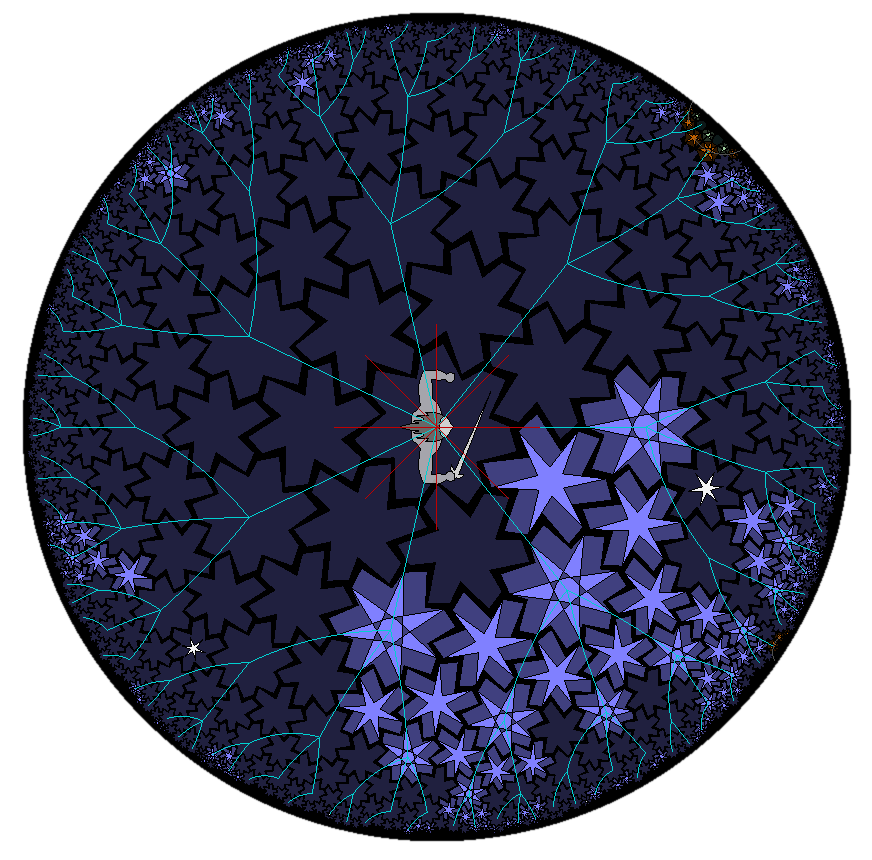
\includegraphics[width=\linewidth]{space-of-programs.png}

\column{0.3\linewidth}
Most programming languages fill the ``space of all possible programs'' because they're Turing complete.

\vspace{0.25 cm}
However, different languages are like different metrics on this space.

\vspace{0.25 cm}
A small change in one is a big change in another.
\end{columns}
\end{frame}

\begin{frame}{Evolution of language choice}
\vspace{0.5 cm}
\begin{block}{High energy physics}
Decades of Fortran, transitioned to C++ in late '90s, may be leaning towards Python now.
\end{block}

\begin{block}{Data science in industry}
Big Data/Hadoop grew out of web development: distributed systems in Java.

\vspace{0.25 cm}
Now involves more machine learning and statistics, so shift toward Scala on the JVM, Python for Scikit-Learn, and R.
\end{block}

\vspace{0.5 cm}
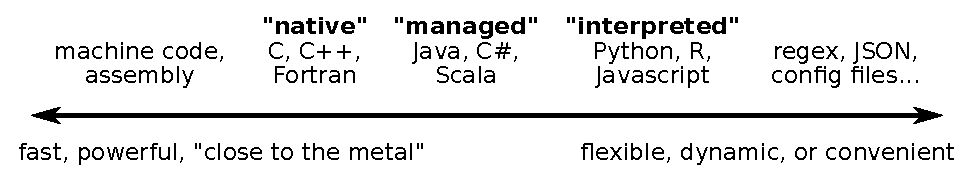
\includegraphics[width=\linewidth]{languages1.pdf}
\end{frame}

\begin{frame}{Abstractions {\it versus} performance?}
\vspace{0.5 cm}
Experience tells us that low-level is fast and high-level is slow.

\vspace{0.5 cm}
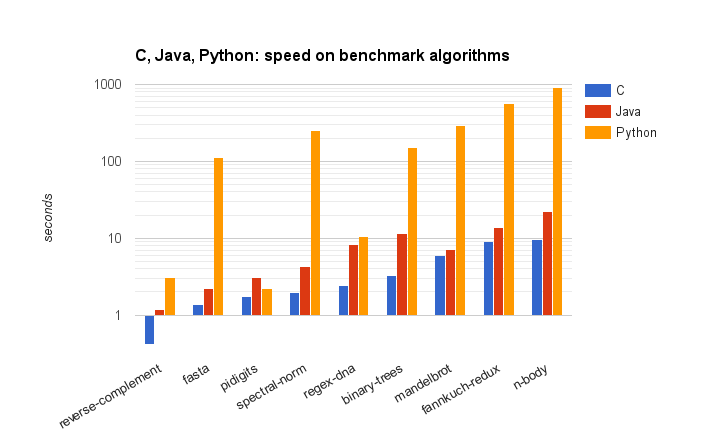
\includegraphics[width=\linewidth]{benchmark-games.png}
\end{frame}

\begin{frame}{Domain-Specific Languages (DSLs)}

\vspace{0.5 cm}
\begin{columns}
\column{0.7\linewidth}
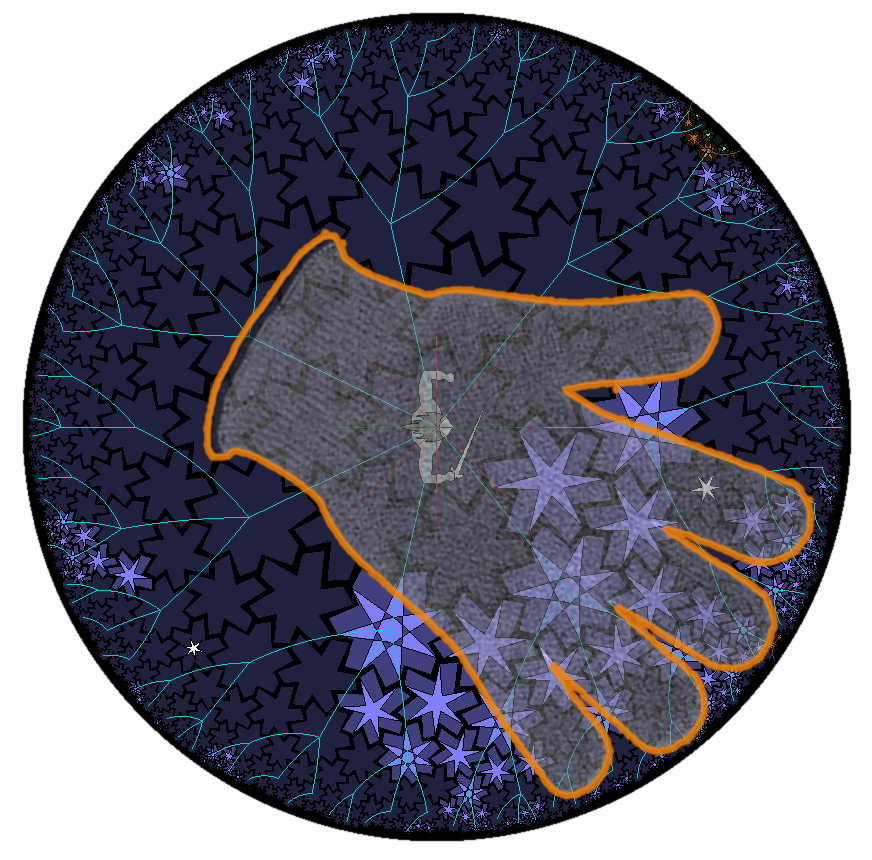
\includegraphics[width=\linewidth]{space-of-programs-glove.png}

\column{0.4\linewidth}
But it doesn't have to be: intentionally restricting the scope of the language allows more optimization.

\vspace{0.25 cm}
\textcolor{darkblue}{Prime example: SQL.}

\vspace{0.25 cm}
But also:
\begin{itemize}
\item Fortran's lack of (aliasable) pointers
\item regular expressions for string manipulation
\item Numpy in Python
\item Histogrammar\ldots
\end{itemize}
\end{columns}
\end{frame}

\begin{frame}{More accurate statement}

\vfill
High-level abstractions $+$ complete generality is slow.

\vfill
High-level abstractions $+$ restricted domain
\begin{itemize}
\item can be as fast as a custom-tuned program \mbox{(especially with JIT),\hspace{-1 cm}}
\item but with better separation of domain knowledge from computing details.
\end{itemize}

\vfill
\begin{uncoverenv}<2>
A well-designed DSL can encourage exploration of the problem space (physics) while the backend optimizes performance.

\vspace{0.25 cm}
(A poorly designed DSL can make it impossible to get work done!)
\end{uncoverenv}
\end{frame}

\begin{frame}{Goals for my future project}
\vfill
I plan to design a domain specific language for end-user physics analysis scripts with the following properties:

\vspace{0.2 cm}
\begin{itemize}
\item a subset of or based on Python syntax
\item non-exclusive: mix with normal (slow) Python
\item immutable, maybe total-functional (next slide)
\item very strongly typed, but only through inference (next$^2$ slide)
\item manual optimizations via CSS-style selectors (next$^3$ slide)
\item supporting imperative idioms through patterns (next$^4$ slide)
\end{itemize}

\vfill
Histogrammar, my histogram-aggregation tool, is a step toward this, which I'm using to test components of the larger-scope project.
\end{frame}

\begin{frame}{Immutable, maybe total-functional}
\vfill
``Functional programming'' eliminates mutable program state:
\begin{itemize}
\item output of functions depend strictly on their inputs
\item {\tt \small x = x + 1} is a false mathematical statement
\item assignments form a time-independent graph, may be written in any order and backend may execute in any order
\item backend may substitute mutable data structures by analyzing (or temporally rearranging) the assignment graph
\item good for concurrency (no locks)
\end{itemize}

\vfill
\begin{uncoverenv}<2->
``Total functional programming'' also eliminates unbounded loops and exceptions:
\begin{itemize}
\item programs are known to halt (not Turing complete), maybe even with time estimates
\item exactly model mathematical functions: $f: \mathcal{D} \to \mathcal{R}$
\end{itemize}
\end{uncoverenv}
\end{frame}

\begin{frame}[fragile]{Strongly typed through inference}
\vfill
Type check is a formal proof that program is free of certain errors.

\vfill
Scala example (eliminates runtime null pointer exceptions):
\begin{lstlisting}[language=scala]
val numberOrNone: Option[Double] = Some(3.14)
val cosx = numberOrNone match {
  case Some(x) => cos(x)
  case None => -999.0
}

// or better
val cosxOrNone = numberOrNone.map(cos(_))

// but cos(numberOrNone) would be a compiler error
\end{lstlisting}
\end{frame}

\begin{frame}{Strongly typed through inference}
\vspace{0.3 cm}
\begin{itemize}
\item<1-> {\tt \small numberOrNone} is a value from the set $\Bbb{R} \cup \{\mbox{\tt \small None}\}$.

\item<2-> One could catch division-by-zero errors in the same way by considering sets like $\Bbb{R} \cup \{-\infty, \infty\}$.

\item<3-> For physics applications, it could be useful to consider any interval, like $(-3, 8] \cap \Bbb{Z}$ or $[0, \infty)$, as ``data types.''
\begin{itemize}
\item<4-> This is like an extreme form of {\tt \small int} versus {\tt \small unsigned int}.
\item<4-> Useful feedback to the data analyst: ``Why does my function output have such a large range?''
\item<4-> Could even be used to set bit widths for a FPGA backend.
\item<4-> I have implemented this for $+$, $-$, $*$, $/$, $**$, and modular arithmetic with 6k lines of unit tests. Extending to continuous functions will involve searches for inflection points.
\end{itemize}
\item<5-> Inference only: intervals specified on input arguments, everything else inferred. The compiler should be telling the user what the domains are, not the other way around. (Being purely functional helps this.)
\end{itemize}
\end{frame}

\begin{frame}{Optimizations via CSS-style selectors}
\end{frame}

\begin{frame}{Imperative idioms through patterns}
\end{frame}

\end{document}
